\documentclass[aspectratio=169,11pt]{beamer}

% ================================================================
% "TABIIY TILNI QAYTA ISHLASH" KURSI
% MA'RUZA 4 --- Masofaga asoslangan qidiruv va imlo tuzatish usullari
%              (d04_qidiruv_imlo.tex)
% Arxetiplar: [A][B][C][D][E] + [F][G][H][I][J][K][L] tarqalgan +
%             [M][N][O][P][Q][R] + ilova [S]
% Rendered slayd soni: ~27 (standart 22-28; 1-haftaning yakuniy ma'ruzasi)
% Qulflangan [I3]: edit_distance("qo'l","ko'l")=1, ("dastur","dastir")=1
%   --- P4 (Day 5) birinchi assert manbayi (course_map hand_example).
% ================================================================

% ================================================================
% RANGLAR  (asl fayldan o'zgarishsiz)
% ================================================================
\definecolor{cnublue}{rgb}{0.07,0.14,0.62}
\definecolor{cnubluelight}{rgb}{0.18,0.30,0.72}
\definecolor{cnubluebg}{rgb}{0.90,0.92,0.97}
\definecolor{deepblue}{rgb}{0.07,0.14,0.62}
\definecolor{deepred}{rgb}{0.60,0.00,0.00}
\definecolor{deepgreen}{rgb}{0.00,0.45,0.00}
\definecolor{halfgray}{gray}{0.55}

% ================================================================
% BEAMER MAVZU --- Boadilla + maxsus footer  (asl fayldan o'zgarishsiz)
% ================================================================
\usetheme{Boadilla}

\setbeamercolor{structure}{fg=cnublue}
\setbeamercolor{frametitle}{bg=cnublue,fg=white}
\setbeamercolor{title}{bg=cnublue,fg=white}
\setbeamercolor{block title}{bg=cnublue,fg=white}
\setbeamercolor{block body}{bg=cnubluebg,fg=black}
\setbeamercolor{alerted text}{fg=deepred}
\setbeamercolor{author in head/foot}{bg=cnubluelight,fg=white}
\setbeamercolor{section in head/foot}{bg=cnublue,fg=white}
\setbeamercolor{page number in head/foot}{bg=cnubluelight,fg=white}

\setbeamertemplate{mini frame}{}
\setbeamertemplate{mini frame in current section}{}
\setbeamertemplate{mini frame in current subsection}{}
\setbeamertemplate{headline}{}
\setbeamertemplate{navigation symbols}{}

\setbeamertemplate{footline}{%
  \leavevmode%
  \hbox{%
    \begin{beamercolorbox}[wd=0.17\paperwidth,ht=2.5ex,dp=1.25ex,leftskip=0.5em]{author in head/foot}%
      \usebeamerfont{author in head/foot}\scriptsize\insertshortauthor%
    \end{beamercolorbox}%
    \begin{beamercolorbox}[wd=0.69\paperwidth,ht=2.5ex,dp=1.25ex,center]{section in head/foot}%
      \usebeamerfont{section in head/foot}%
      \scriptsize\insertsectionnavigationhorizontal{0.69\paperwidth}{}{}%
    \end{beamercolorbox}%
    \begin{beamercolorbox}[wd=0.14\paperwidth,ht=2.5ex,dp=1.25ex,rightskip=0.5em]{page number in head/foot}%
      \hfill\scriptsize\color{white}%
      \insertframenumber{}/\inserttotalframenumber%
    \end{beamercolorbox}%
  }%
  \vskip0pt%
}

% ================================================================
% PAKETLAR  (asl fayldan o'zgarishsiz)
% ================================================================
\usepackage[utf8]{inputenc}
\usepackage[T1]{fontenc}
\usepackage{lmodern}
\usepackage{amsmath,amssymb}
\usepackage{booktabs}
\usepackage{xcolor}
\usepackage{listings}
\lstset{
    language=Python,
    basicstyle=\ttfamily\scriptsize,
    keywordstyle=\bfseries\color{deepblue},
    emphstyle=\ttfamily\color{deepred},
    stringstyle=\color{deepgreen},
    commentstyle=\itshape\color{halfgray},
    numbers=left,
    numberstyle=\scriptsize\color{halfgray},
    rulesepcolor=\color{cnublue!30},
    frame=shadowbox,
    breaklines=true,
    showstringspaces=false,
    tabsize=2
}
\usepackage{tcolorbox}
\tcbuselibrary{skins}
\tcbset{
  defbox/.style={colback=cnubluebg,colframe=cnublue,
                 fonttitle=\small\bfseries\color{white},
                 attach boxed title to top left={yshift=-2mm,xshift=4mm},
                 boxed title style={colback=cnublue,colframe=cnublue}},
  warnbox/.style={colback=orange!8,colframe=orange!70!black,
                  fonttitle=\small\bfseries},
  okbox/.style={colback=green!7,colframe=green!55!black,
                fonttitle=\small\bfseries}
}
\usepackage{tikz}
\usetikzlibrary{arrows.meta,positioning}

% ================================================================
% QO'SHIMCHALAR  (asl fayldan o'zgarishsiz)
% ================================================================
\AtBeginSection[]{%
  \begin{frame}{Prezentatsiya rejasi}
    \tableofcontents[currentsection]
  \end{frame}}

\newcommand{\bunda}[1]{{\small\textbf{bunda:}\; #1}}
\newcommand{\bajarildi}{{\color{deepgreen}\large$\checkmark$}\;}

% ================================================================
% METAMA'LUMOT
% ================================================================
\title[Qidiruv va imlo tuzatish]{Masofaga asoslangan qidiruv va imlo tuzatish}
\subtitle{Tabiiy tilni qayta ishlash --- 4-ma'ruza}
\author[A.A.\,Abdulali]{A.A.\,Abdulali}
\date{19-iyun 2026}
\institute{11:00--12:20 \quad$\cdot$\quad mavzu \textnumero{}4}

% ================================================================
\begin{document}
% ================================================================

% ----------------------------------------------------------------
% [A] TITUL
% ----------------------------------------------------------------
\maketitle

% ================================================================
\section[Kirish]{Kirish: o'xshashlikdan qidiruv va tuzatishgacha}
% ================================================================

% ----------------------------------------------------------------
% [B] TAKRORLASH: L3 va bugungi P3
% ----------------------------------------------------------------
\begin{frame}{Takrorlash: o'xshashlikni qanday o'lchagandik?}
  \begin{columns}[T]
    \begin{column}{0.49\textwidth}
      \begin{tcolorbox}[warnbox,title=1-savol]
        \small
        L3 da ikki vektor (yoki so'z) o'xshashligini qaysi o'lchov bilan
        baholadik?\\[3pt]
        \footnotesize Qiymat oralig'i qanday edi?
      \end{tcolorbox}
    \end{column}
    \begin{column}{0.49\textwidth}
      \begin{tcolorbox}[warnbox,title=2-savol]
        \small
        Bugun ertalab P3 da \texttt{most\_similar} eng o'xshash so'zni
        topdi. U \textbf{nechta} so'z bilan solishtirdi?
      \end{tcolorbox}
    \end{column}
  \end{columns}
  \pause
  \vspace{4pt}
  \begin{columns}[T]
    \begin{column}{0.49\textwidth}
      \begin{tcolorbox}[okbox,title=1-javob]
        \small
        \textbf{Kosinus o'xshashligi}, oralig'i $[0,1]$
        (TF-IDF/embedding uchun).
      \end{tcolorbox}
    \end{column}
    \begin{column}{0.49\textwidth}
      \begin{tcolorbox}[okbox,title=2-javob]
        \small
        \textbf{Hammasi bilan!} Lug'atdagi har bir so'z bilan --- ya'ni
        $O(N)$.\\
        \footnotesize\textcolor{halfgray}{Millionlab hujjatda bu sekin. Bugun tezlatamiz.}
      \end{tcolorbox}
    \end{column}
  \end{columns}
\end{frame}

% ----------------------------------------------------------------
% [C] BUGUNGI MAQSADLAR
% ----------------------------------------------------------------
\begin{frame}{Siz bugungi dars oxirida quyidagilarni bajara olasiz:}
  \begin{enumerate}\setlength\itemsep{6pt}
    \item \textbf{Keltirib chiqara olasiz:} tahrir masofasi (Levenshtein)
          dinamik dasturlash rekurrensiyasini.
    \item \textbf{Qo'lda hisoblay olasiz:} kichik so'zlar uchun tahrir
          masofasini DP jadvali bilan ($\text{edit}(\texttt{qo'l},\texttt{ko'l})=1$).
    \item \textbf{Qo'llay olasiz:} noisy channel modeli ---
          $\arg\max_w P(x{\mid}w)P(w)$ bilan eng ehtimoliy tuzatishni topish.
    \item \textbf{Taqqoslay olasiz:} aniq qidiruv (k-NN) va taxminiy
          qidiruv (LSH) --- qachon qaysi biri.
  \end{enumerate}
  \vspace{4pt}
  \begin{tcolorbox}[defbox,title=Oldindan talab]
    \footnotesize
    L1 dan: tokenizatsiya, apostrof muammosi. L2 dan: ehtimollik,
    $\arg\max$. L3 dan: o'xshashlik tushunchasi. Matematikadan: matritsa,
    minimum.
  \end{tcolorbox}
\end{frame}

% ----------------------------------------------------------------
% [D] REJA VA VAQT BYUDJETI
% ----------------------------------------------------------------
\begin{frame}{Bugungi dars rejasi:}
  \begin{center}
  \small
  \begin{tabular}{c p{5.0cm} c p{3.2cm}}
    \toprule
    \textbf{Blok}& \textbf{Mavzu} & \textbf{Vaqt} & \textbf{Hosil bo'luvchi natija}\\
    \midrule
    1 & Tez o'xshashlik qidiruvi: KNN, LSH & 18 daq & Jaccard, LSH tushunchasi \\
    2 & Imlo tuzatish: noisy channel & 16 daq & $\arg\max P(x{\mid}w)P(w)$ \\
    3 & Tahrir masofasi (Levenshtein) + DP & 26 daq & Qo'lda hisoblangan DP jadval \\
    4 & Tizim arxitekturasi & 10 daq & To'liq tuzatish quvuri \\
    \midrule
      & Xulosa va 4-amaliyotga ko'rsatmalar & 10 daq & Ertaga nima qurishingiz \\
    \bottomrule
  \end{tabular}
  \end{center}
  \vspace{4pt}
  \begin{tcolorbox}[warnbox,title=Bu dars 1-haftaning yakuni]
    \footnotesize\sloppy
    Tozalash (m01) $\to$ tasniflash (m02) $\to$ embedding (m03) $\to$
    \textbf{qidiruv va tuzatish (m04)}. Bugungi $\text{edit}(\texttt{qo'l},\texttt{ko'l})=1$
    ertangi amaliyotda \texttt{assert} bo'ladi.
  \end{tcolorbox}
\end{frame}

% ----------------------------------------------------------------
% [E] MUAMMO BIRINCHI
% ----------------------------------------------------------------
\begin{frame}{Bugungi dars uchun muammo: foydalanuvchi ``telfon'' deb yozsa, aniq moslik topilmaydi}
  \begin{columns}[T]
    \begin{column}{0.50\textwidth}
      \textbf{Ikki real muammo:}\\[4pt]
      \small
      \begin{tcolorbox}[warnbox,title=1. Imlo xatosi,top=2pt,bottom=2pt]
        \footnotesize
        Qidiruvda \texttt{"telfon"} yozildi.\\
        Lug'atda \texttt{"telefon"} bor.\\
        Aniq (exact) moslik $\Rightarrow$ \alert{0 natija}.\\
        \textbf{Qaysi so'z nazarda tutilgan?}
      \end{tcolorbox}
      \vspace{3pt}
      \begin{tcolorbox}[warnbox,title=2. Sekin qidiruv,top=2pt,bottom=2pt]
        \footnotesize
        Million hujjat orasidan eng o'xshashini topish:
        har biriga kosinus $\Rightarrow$ $O(N)$, juda sekin.
      \end{tcolorbox}
    \end{column}
    \begin{column}{0.46\textwidth}
      \textbf{Bugungi yechimlar:}\\[4pt]
      \small
      \begin{enumerate}\setlength\itemsep{4pt}
        \item \textbf{Tahrir masofasi} + \textbf{noisy channel}:
              eng ehtimoliy to'g'ri so'zni topadi.
        \item \textbf{LSH}: o'xshash hujjatlarni bir ``savat''ga
              tushiradi $\Rightarrow$ qidiruv tez.
      \end{enumerate}
      \vspace{5pt}
      \begin{tcolorbox}[okbox,top=2pt,bottom=2pt]
        \footnotesize
        Ikkalasi ham \textbf{taxminiy} (approximate) usullar ---
        aniqlikni tezlik va moslashuvchanlikka almashtiradi.
      \end{tcolorbox}
    \end{column}
  \end{columns}
\end{frame}

% ================================================================
\section[Tez qidiruv]{Tez o'xshashlik qidiruvi: LSH}
% ================================================================

% ----------------------------------------------------------------
% [F1] INTUITSIYA: KNN sekin, LSH tez
% ----------------------------------------------------------------
\begin{frame}{Intuitsiya: o'xshashlarni avval ``savatlarga'' ajratamiz}
  \begin{columns}[T]
    \begin{column}{0.50\textwidth}
      \textbf{Aniq qidiruv (k-NN):}\\[3pt]
      \small
      So'rovni \textbf{barcha} $N$ hujjat bilan solishtiramiz
      $\Rightarrow O(N)$. 1\,000 hujjatda --- mayli; million hujjatda --- sekin.\\[6pt]
      \textbf{LSH g'oyasi:}\\[3pt]
      O'xshash hujjatlar \textbf{katta ehtimol bilan} bir xil ``savat''
      (bucket) ga tushadigan xesh quramiz. So'rov uchun faqat
      \textbf{o'sha savatni} tekshiramiz.
    \end{column}
    \begin{column}{0.46\textwidth}
      \begin{center}
      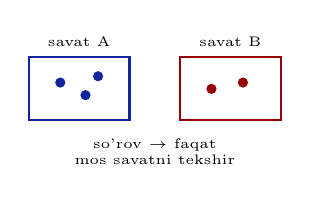
\begin{tikzpicture}[scale=0.8]
        \draw[draw=cnublue,thick] (0,0) rectangle (1.6,1.0);
        \node[font=\tiny] at (0.8,1.25) {savat A};
        \node[circle,fill=cnublue,inner sep=1.3pt] at (0.5,0.6) {};
        \node[circle,fill=cnublue,inner sep=1.3pt] at (0.9,0.4) {};
        \node[circle,fill=cnublue,inner sep=1.3pt] at (1.1,0.7) {};
        \draw[draw=deepred,thick] (2.4,0) rectangle (4.0,1.0);
        \node[font=\tiny] at (3.2,1.25) {savat B};
        \node[circle,fill=deepred,inner sep=1.3pt] at (2.9,0.5) {};
        \node[circle,fill=deepred,inner sep=1.3pt] at (3.4,0.6) {};
        \node[font=\tiny,align=center] at (2.0,-0.5)
          {so'rov $\to$ faqat\\ mos savatni tekshir};
      \end{tikzpicture}
      \end{center}
      \footnotesize\color{halfgray}
      Solishtirishlar soni $O(N)$ dan savat hajmiga tushadi ---
      amalda subchiziqli (sublinear).
    \end{column}
  \end{columns}
\end{frame}

% ----------------------------------------------------------------
% [G1] RASMIY TA'RIF: Jaccard, shingling, MinHash, LSH + BUNDA
% ----------------------------------------------------------------
\begin{frame}{Jaccard o'xshashligi, MinHash va LSH: rasmiy ta'rif}
  \begin{tcolorbox}[defbox,title=Ta'rif: Jaccard o'xshashligi]
    \vspace{-0.4em}
    $$ J(A,B) = \frac{|A \cap B|}{|A \cup B|} \in [0,1] $$
  \end{tcolorbox}
  \vspace{3pt}
  \bunda{$A,B$ --- hujjatning \textit{shingle} (so'z yoki $k$-belgi
  bo'laklari) to'plamlari; $|A\cap B|$ --- umumiy bo'laklar soni;
  $|A\cup B|$ --- jami noyob bo'laklar.}
  \vspace{5pt}
  \begin{itemize}\small\setlength\itemsep{3pt}
    \item \textbf{MinHash}: tasodifiy permutatsiya bo'yicha minimal element ---
          $P[\text{minhash}(A){=}\text{minhash}(B)] = J(A,B)$.
    \item \textbf{LSH}: MinHash imzosini $b$ ``band''ga bo'lib, har bandni
          savatga xeshlaymiz; bitta bandda mos kelsa --- nomzod.
    \item Natija: Jaccard yuqori juftlar bir savatga tushish ehtimoli yuqori.
  \end{itemize}
\end{frame}

% ----------------------------------------------------------------
% [I1] QO'LDA HISOB: Jaccard
% ----------------------------------------------------------------
\begin{frame}{Qo'lda hisob: ikki hujjatning Jaccard o'xshashligi}
  \begin{tcolorbox}[defbox,title=Kichik misol (so'z to'plamlari)]
    \small
    $A = \{$\texttt{nlp}, \texttt{juda}, \texttt{qiziq}$\}$\qquad
    $B = \{$\texttt{nlp}, \texttt{juda}, \texttt{foydali}$\}$
  \end{tcolorbox}
  \vspace{0.2em}
  \begin{columns}[T]
    \begin{column}{0.52\textwidth}
      \textbf{Hisoblaymiz:}
      \begin{align*}
        A \cap B &= \{\texttt{nlp}, \texttt{juda}\} \Rightarrow |A\cap B| = 2\\
        A \cup B &= \{\texttt{nlp}, \texttt{juda}, \texttt{qiziq}, \texttt{foydali}\}\\
                 &\Rightarrow |A\cup B| = 4
      \end{align*}
      $$ J(A,B) = \frac{2}{4} = \mathbf{0.5} $$
    \end{column}
    \begin{column}{0.44\textwidth}
      \begin{tcolorbox}[okbox,top=2pt,bottom=2pt]
        \footnotesize
        Eslatma: L3 da \textbf{aynan shu} ikki hujjat uchun
        kosinus $= 2/3 \approx 0.667$ edi.\\[3pt]
        Jaccard \textbf{to'plam} (bor/yo'q), kosinus esa
        \textbf{chastota} bilan ishlaydi --- shuning uchun farq.
      \end{tcolorbox}
    \end{column}
  \end{columns}
\end{frame}

% ================================================================
\section[Imlo tuzatish]{Imlo tuzatish: noisy channel va tahrir masofasi}
% ================================================================

% ----------------------------------------------------------------
% [G2] RASMIY TA'RIF: Noisy channel + BUNDA
% ----------------------------------------------------------------
\begin{frame}{Noisy channel modeli: eng ehtimoliy to'g'ri so'z}
  \textbf{Intuitsiya:} foydalanuvchi to'g'ri so'z $w$ ni o'ylagan, lekin
  ``shovqinli kanal'' (klaviatura, e'tiborsizlik) uni xato $x$ ga aylantirgan.
  Biz $x$ ni ko'rib, $w$ ni tiklamoqchimiz.
  \vspace{3pt}
  \begin{tcolorbox}[defbox,title=Ta'rif: noisy channel imlo tuzatish]
    \vspace{-0.4em}
    $$ \hat{w} = \arg\max_{w \in V} P(w \mid x)
       = \arg\max_{w \in V} \; \underbrace{P(x \mid w)}_{\text{xato modeli}}\;
                                \underbrace{P(w)}_{\text{til modeli}} $$
  \end{tcolorbox}
  \vspace{2pt}
  \bunda{$x$ --- kuzatilgan (xato) so'z; $w$ --- nomzod to'g'ri so'z;
  $P(w)$ --- unigram chastota (so'z qanchalik keng tarqalgan);
  $P(x{\mid}w)$ --- $w$ dan $x$ ga xato qilish ehtimoli.}
  \vspace{4pt}
  \footnotesize
  Nomzodlar $V$ --- $x$ ga \textbf{tahrir masofasi kichik} so'zlar
  (odatda $\le 2$). Bu masofani keyin DP bilan aniq hisoblaymiz.
\end{frame}

% ----------------------------------------------------------------
% [I2] QO'LDA HISOB: Noisy channel ranking
% ----------------------------------------------------------------
\begin{frame}{Qo'lda hisob: ``kitop'' ni qanday tuzatamiz?}
  \begin{tcolorbox}[defbox,title=Kuzatilgan xato: x = ``kitop'']
    \small
    Ikki nomzod (tahrir masofasi $=1$): \texttt{kitob} va \texttt{kotib}.
  \end{tcolorbox}
  \vspace{0.2em}
  \begin{columns}[T]
    \begin{column}{0.54\textwidth}
      \small
      \begin{tabular}{lccc}
        \toprule
        Nomzod $w$ & $P(w)$ & $P(x{\mid}w)$ & ko'paytma \\
        \midrule
        \texttt{kitob} & 0.80 & 0.10 & $\mathbf{0.080}$ \\
        \texttt{kotib} & 0.10 & 0.02 & $0.002$ \\
        \bottomrule
      \end{tabular}
      \vspace{6pt}
      $$ \hat{w} = \arg\max = \texttt{kitob} \quad (0.080 > 0.002) $$
    \end{column}
    \begin{column}{0.42\textwidth}
      \begin{tcolorbox}[okbox,top=2pt,bottom=2pt]
        \footnotesize
        Ikkala nomzod ham $x$ ga bir xil yaqin (masofa 1), lekin
        \texttt{kitob} \textbf{keng tarqalgan} ($P(w)$ yuqori) ---
        shuning uchun u g'olib. Til modeli muhim!
      \end{tcolorbox}
    \end{column}
  \end{columns}
\end{frame}

% ----------------------------------------------------------------
% [G3] RASMIY TA'RIF: Levenshtein + DP rekurrensiya + BUNDA
% ----------------------------------------------------------------
\begin{frame}{Tahrir masofasi (Levenshtein): rasmiy ta'rif}
  \textbf{Intuitsiya:} bir so'zni boshqasiga aylantirish uchun zarur
  \textbf{minimal} amallar soni. Uch amal: qo'shish, o'chirish, almashtirish.
  \begin{tcolorbox}[defbox,title=Ta'rif: DP rekurrensiyasi]
    \vspace{-0.3em}
    $$ D[i][j] =
       \begin{cases}
         D[i{-}1][j{-}1], & \text{agar } s_1[i]=s_2[j]\\[3pt]
         1 + \min\big(D[i{-}1][j],\, D[i][j{-}1],\, D[i{-}1][j{-}1]\big), & \text{aks holda}
       \end{cases} $$
  \end{tcolorbox}
  \vspace{2pt}
  \bunda{$D[i][j]$ --- $s_1$ ning birinchi $i$, $s_2$ ning birinchi $j$
  belgisi orasidagi masofa; uch had mos ravishda \textbf{o'chirish},
  \textbf{qo'shish}, \textbf{almashtirish}.}
  \vspace{3pt}
  \footnotesize Asos: $D[i][0]=i$ (hammasini o'chirish),
  $D[0][j]=j$ (hammasini qo'shish).
\end{frame}

% ----------------------------------------------------------------
% [H3] KELTIRIB CHIQARISH: DP qadamlari
% ----------------------------------------------------------------
\begin{frame}{Keltirib chiqarish: nega aynan shu uch had?}
  \textbf{1-qadam.} $D[i][j]$ ni hisoblashda oxirgi belgilarni qaraymiz:
  $s_1[i]$ va $s_2[j]$.
  \pause
  \textbf{2-qadam.} Agar ular \textbf{teng} bo'lsa --- amal kerak emas,
  masofa $D[i{-}1][j{-}1]$ ga teng.
  \pause
  \textbf{3-qadam.} Aks holda eng arzon amalni tanlaymiz ($1$ narx):
  \begin{itemize}\small\setlength\itemsep{2pt}
    \item $D[i{-}1][j]+1$ --- $s_1[i]$ ni \textbf{o'chirish},
    \item $D[i][j{-}1]+1$ --- $s_2[j]$ ni \textbf{qo'shish},
    \item $D[i{-}1][j{-}1]+1$ --- $s_1[i] \to s_2[j]$ \textbf{almashtirish}.
  \end{itemize}
  \begin{tcolorbox}[okbox,top=2pt,bottom=2pt]
    \small \textbf{Xulosa:} har katak faqat uch qo'shnisiga tayanadi ---
    shuning uchun jadvalni chap-yuqoridan to'ldiramiz; murakkablik $O(mn)$.
  \end{tcolorbox}
\end{frame}

% ----------------------------------------------------------------
% [I3] QO'LDA HISOB --- QULFLANGAN TRACEABILITY SLAYD
%
% P4 (kun-5) birinchi assert bilan solishtiring:
%   edit_distance("qo'l","ko'l") = 1   [Ma'ruza L4 [I3]-slayd]
%   edit_distance("dastur","dastir") = 1
% course_map.yaml hand_example verbatim.
% ----------------------------------------------------------------
\begin{frame}{Qo'lda hisob: edit\_distance(``qo'l'', ``ko'l'') = 1}
  \begin{columns}[T]
    \begin{column}{0.52\textwidth}
      \small DP jadval ($s_1=$\texttt{qo'l}, $s_2=$\texttt{ko'l}):
      \vspace{2pt}
      \begin{center}\footnotesize
      \begin{tabular}{c|ccccc}
         & \texttt{""} & \texttt{k} & \texttt{o} & \texttt{'} & \texttt{l} \\
        \hline
        \texttt{""} & 0 & 1 & 2 & 3 & 4 \\
        \texttt{q}  & 1 & \textbf{1} & 2 & 3 & 4 \\
        \texttt{o}  & 2 & 2 & \textbf{1} & 2 & 3 \\
        \texttt{'}  & 3 & 3 & 2 & \textbf{1} & 2 \\
        \texttt{l}  & 4 & 4 & 3 & 2 & \textbf{1} \\
      \end{tabular}
      \end{center}
    \end{column}
    \begin{column}{0.44\textwidth}
      \textbf{Natija:} $D[4][4] = \mathbf{1}$\\[3pt]
      \footnotesize
      Faqat birinchi belgi farq qiladi: \texttt{q}$\to$\texttt{k}
      (1 almashtirish). Qolgan \texttt{o'l} bir xil.
      \vspace{5pt}
      \begin{tcolorbox}[okbox,title=Ikkinchi tekshiruv,top=2pt,bottom=2pt]
        \footnotesize
        $\text{edit}(\texttt{dastur},\texttt{dastir}) = \mathbf{1}$
        (\texttt{u}$\to$\texttt{i} almashtirish, 5-belgi).
      \end{tcolorbox}
      \vspace{2pt}
      \footnotesize\color{halfgray}
      Ertangi P4 birinchi assert:\\
      \texttt{edit\_distance("qo'l","ko'l")==1}\\
      \textit{\# Ma'ruza L4 [I3]-slayd}
    \end{column}
  \end{columns}
\end{frame}

% ----------------------------------------------------------------
% [J3] SIZNING VAZIFANGIZ: edit distance
% ----------------------------------------------------------------
\begin{frame}{Sizning vazifangiz: tahrir masofasini toping}
  \begin{tcolorbox}[warnbox,title=Savol --- 2 daqiqa]
    \small
    a) $\text{edit}(\texttt{maktab},\, \texttt{maktub}) = ?$\\[4pt]
    b) $\text{edit}(\texttt{kitob},\, \texttt{kitoblar}) = ?$\\[4pt]
    \footnotesize Har biri uchun qaysi amal(lar) ishlatiladi?
  \end{tcolorbox}
  \pause
  \begin{tcolorbox}[okbox,title=Javob]
    \small
    a) $\mathbf{1}$ --- \texttt{a}$\to$\texttt{u} bitta \textbf{almashtirish}
    (4-belgi).\\[3pt]
    b) $\mathbf{3}$ --- \texttt{l}, \texttt{a}, \texttt{r} uchta
    \textbf{qo'shish} (so'z oxiriga).\\[3pt]
    \footnotesize Eslatma: o'zbek qo'shimchalari (\texttt{-lar}, \texttt{-da}\ldots)
    tahrir masofasini oshiradi --- bu [M]-slaydda muhim bo'ladi.
  \end{tcolorbox}
\end{frame}

% ----------------------------------------------------------------
% [K3] KOD <-> FORMULA: edit_distance DP  [fragile]
% ----------------------------------------------------------------
\begin{frame}[fragile]{Kod $\leftrightarrow$ formula: tahrir masofasi DP da}
  \begin{columns}[T]
    \begin{column}{0.56\textwidth}
\begin{lstlisting}
def edit_distance(s1, s2):
    m, n = len(s1), len(s2)
    D = [[0]*(n+1) for _ in range(m+1)]
    for i in range(m+1): D[i][0] = i   # o'chirish
    for j in range(n+1): D[0][j] = j   # qo'shish
    for i in range(1, m+1):
        for j in range(1, n+1):
            if s1[i-1] == s2[j-1]:
                D[i][j] = D[i-1][j-1]
            else:
                D[i][j] = 1 + min(
                    D[i-1][j],     # o'chirish
                    D[i][j-1],     # qo'shish
                    D[i-1][j-1])   # almashtirish
    return D[m][n]

edit_distance("qo'l", "ko'l")      # -> 1
\end{lstlisting}
    \end{column}
    \begin{column}{0.40\textwidth}
      \textbf{Kod $\to$ formula:}\\[3pt]
      \footnotesize
      \begin{tabular}{p{1.9cm}p{2.1cm}}
        \toprule
        Kod & Formula \\
        \midrule
        \texttt{D[i][0]=i} & asos (o'chirish) \\
        \texttt{s1[i-1]==s2[j-1]} & belgilar teng \\
        \texttt{1+min(...)} & 3 amal minimumi \\
        \texttt{D[m][n]} & yakuniy masofa \\
        \bottomrule
      \end{tabular}
      \vspace{4pt}
      \begin{tcolorbox}[okbox,top=2pt,bottom=2pt]
        \footnotesize
        Ertangi P4 da \texttt{m04 SpellLSHRetriever.edit\_distance()}
        aynan shu DP ni amalga oshiradi.
      \end{tcolorbox}
    \end{column}
  \end{columns}
\end{frame}

% ----------------------------------------------------------------
% [L3] CHEKLOVLAR VA TIPIK XATOLAR
% ----------------------------------------------------------------
\begin{frame}{Cheklovlar va tipik xatolar}
  \begin{columns}[T]
    \begin{column}{0.50\textwidth}
      \begin{tcolorbox}[warnbox,title=Usulning cheklovlari]
        \small
        \begin{itemize}\setlength\itemsep{2pt}
          \item Levenshtein \textbf{ma'noni} bilmaydi:
                \texttt{ot} va \texttt{it} masofasi 1, lekin ma'no boshqa.
          \item Nomzodlar soni masofa $\le 2$ da ham katta ---
                hammasini tekshirish sekin.
          \item LSH \textbf{taxminiy}: o'xshash juft boshqa savatga
                tushib, e'tibordan chetda qolishi mumkin (false negative).
        \end{itemize}
      \end{tcolorbox}
    \end{column}
    \begin{column}{0.46\textwidth}
      \begin{tcolorbox}[warnbox,title=Tipik xato]
        \small
        Asos qatorini unutish:\\
        \footnotesize
        \texttt{D[i][0]=i} va \texttt{D[0][j]=j} qo'yilmasa, bo'sh
        satrga masofa noto'g'ri ($0$) bo'lib, butun jadval buziladi.\\[4pt]
        \normalsize Asos qatorlar --- DP ning poydevori.
      \end{tcolorbox}
      \vspace{3pt}
      \footnotesize\color{halfgray}
      Tezlashtirish: nomzodlarni avval LSH/lug'at-trie bilan
      filtrlash, keyin aniq masofani hisoblash.
    \end{column}
  \end{columns}
\end{frame}

% ----------------------------------------------------------------
% [G4] SUBITEM 4: avtomatik tuzatish tizimi arxitekturasi
% ----------------------------------------------------------------
\begin{frame}{Avtomatik tuzatish tizimi: komponentlar va oqim}
  \begin{center}
  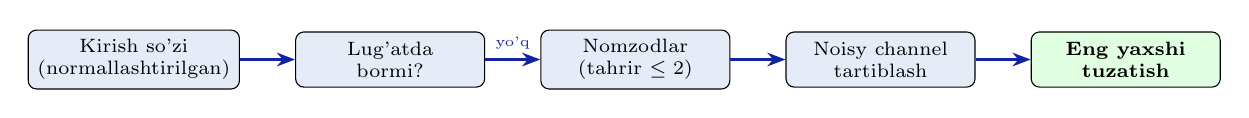
\begin{tikzpicture}[
      box/.style={draw, fill=cnubluebg, rounded corners=3pt,
                  minimum width=2.4cm, minimum height=0.7cm,
                  font=\scriptsize, align=center},
      fin/.style={draw, fill=green!12, rounded corners=3pt,
                  minimum width=2.4cm, minimum height=0.7cm,
                  font=\scriptsize\bfseries, align=center},
      arr/.style={-{Stealth}, thick, color=cnublue}
  ]
    \node[box] (in)  {Kirish so'zi\\ (normallashtirilgan)};
    \node[box, right=0.7cm of in]  (dict) {Lug'atda\\ bormi?};
    \node[box, right=0.7cm of dict] (cand) {Nomzodlar\\ (tahrir $\le 2$)};
    \node[box, right=0.7cm of cand] (rank) {Noisy channel\\ tartiblash};
    \node[fin, right=0.7cm of rank] (out)  {Eng yaxshi\\ tuzatish};
    \draw[arr] (in)--(dict);
    \draw[arr] (dict)--(cand) node[midway,above,font=\tiny]{yo'q};
    \draw[arr] (cand)--(rank);
    \draw[arr] (rank)--(out);
  \end{tikzpicture}
  \end{center}
  \vspace{2pt}
  \begin{columns}[T]
    \begin{column}{0.50\textwidth}
      \footnotesize
      \textbf{Komponentlar:}
      \begin{enumerate}\setlength\itemsep{1pt}
        \item Normallashtirish (apostrof, kichik harf) --- m01
        \item Lug'at tekshiruvi (bor bo'lsa --- tuzatish shart emas)
        \item Nomzod generatsiyasi (tahrir masofasi)
        \item Tartiblash (noisy channel: $P(x{\mid}w)P(w)$)
      \end{enumerate}
    \end{column}
    \begin{column}{0.46\textwidth}
      \begin{tcolorbox}[okbox,title=Hujjat qidiruvi uchun,top=2pt,bottom=2pt]
        \footnotesize
        Katta korpusda o'xshash hujjatni topish uchun shu quvurga
        \textbf{MinHash LSH indeks} qo'shiladi --- m04 da ikkalasi birga
        keladi.
      \end{tcolorbox}
    \end{column}
  \end{columns}
\end{frame}

% ================================================================
\section[Xulosa]{Xulosa va amaliyotga ko'prik}
% ================================================================

% ----------------------------------------------------------------
% [M] O'ZBEK TILIGA XOSLIK (majburiy arxetip)
% ----------------------------------------------------------------
\begin{frame}{O'zbek tilida: apostrof va qo'shimchalar tahrir masofasini chalg'itadi}
  \begin{columns}[T]
    \begin{column}{0.50\textwidth}
      \textbf{1. Apostrof muammosi:}\\[3pt]
      \small
      \begin{tabular}{ll}
        \toprule
        Juft & edit \\
        \midrule
        \texttt{yo'l} vs \texttt{yol}     & 1 \\
        \texttt{to'g'ri} vs \texttt{togri} & 2 \\
        \bottomrule
      \end{tabular}\\[4pt]
      \footnotesize
      Apostrof tushib qolsa, bir xil so'z ``xato'' ko'rinadi.
      Yana ASCII \texttt{'} va U+2019 \texttt{'} --- byte-darajada
      \textbf{turli} belgilar (L1 dan eslang).
    \end{column}
    \begin{column}{0.46\textwidth}
      \textbf{2. Agglutinatsiya:}\\[3pt]
      \small
      \texttt{kitob}, \texttt{kitobni}, \texttt{kitobimizdan} ---
      bir o'zak, lekin o'zaro tahrir masofasi katta.\\[4pt]
      \begin{tcolorbox}[warnbox,title=Oqibat,top=2pt,bottom=2pt]
        \footnotesize
        Nomzodlar fazosi ulkanlashadi; lug'at har bir qo'shimchali
        shaklni o'z ichiga ololmaydi $\Rightarrow$ OOV.
      \end{tcolorbox}
      \vspace{2pt}
      \footnotesize\textbf{Yechim:} masofadan oldin \textbf{normallashtirish}
      (apostrof + stem, m01) --- xato signalini kamaytiradi.
    \end{column}
  \end{columns}
\end{frame}

% ----------------------------------------------------------------
% [N] SINTEZ: 1-hafta yoyi + usullar taqqoslovi
% ----------------------------------------------------------------
\begin{frame}{Sintez: 1-haftada o'xshashlikni uch darajada o'lchadik}
  \begin{center}\small
  \begin{tabular}{p{2.8cm}p{3.4cm}p{4.4cm}}
    \toprule
    \textbf{Usul} & \textbf{Nimani o'lchaydi} & \textbf{Qachon} \\
    \midrule
    Levenshtein & Belgi-darajasi (imlo) & Imlo tuzatish, yaqin so'z \\
    Jaccard + LSH & To'plam (bor/yo'q) & Yaqin-nusxa hujjat, tez qidiruv \\
    Kosinus + embedding & Vektor (ma'no) & Semantik o'xshashlik (L3) \\
    \bottomrule
  \end{tabular}
  \end{center}
  \vspace{4pt}
  \begin{tcolorbox}[okbox,title=1-hafta kapstone yoyi,top=2pt,bottom=2pt]
    \footnotesize
    \textbf{m01} tozalash $\to$ \textbf{m02} TF-IDF tasniflash $\to$
    \textbf{m03} embedding o'xshashlik $\to$ \textbf{m04} imlo tuzatish + LSH qidiruv.
    To'rt modul birgalikda --- hujjat yordamchingizning klassik yadrosi.
    2-haftada neyron usullarga o'tamiz.
  \end{tcolorbox}
\end{frame}

% ----------------------------------------------------------------
% [O] SEMINAL MANBA + MUHOKAMA SAVOLI
% ----------------------------------------------------------------
\begin{frame}{Seminal manba: Norvig (2009)}
  \begin{tcolorbox}[defbox,title=Manba]
    \small
    Norvig, P.\ (2009). \textbf{How to Write a Spelling Corrector.}
    \textit{norvig.com/spell-correct.html}
  \end{tcolorbox}
  \vspace{5pt}
  \textbf{Asosiy g'oya:}
  \begin{itemize}\small\setlength\itemsep{3pt}
    \item 21 qatorlik Python: noisy channel + tahrir masofasi + unigram LM.
    \item Nomzodlar --- tahrir masofasi $1$ va $2$ dagi so'zlar.
    \item $P(w)$ katta korpus chastotasidan; $P(x{\mid}w)$ soddalashtirilgan.
  \end{itemize}
  \vspace{5pt}
  \begin{tcolorbox}[warnbox,title=Muhokama savoli (P4 gacha o'ylang)]
    \small
    Norvig faqat tahrir masofasi $\le 2$ nomzodlarni ko'radi.
    O'zbek agglutinativ so'zlari (\texttt{kitobimizdan}) uchun bu
    \textbf{yetarlimi}? Nima qo'shish kerak?
  \end{tcolorbox}
\end{frame}

% ----------------------------------------------------------------
% [P] MAQSADLAR BAJARILDI
% ----------------------------------------------------------------
\begin{frame}{Bugungi maqsadlar bajarildi}
  \begin{enumerate}\setlength\itemsep{8pt}
    \item \bajarildi \textbf{Keltirib chiqardik:} Levenshtein DP
          rekurrensiyasi --- uch amal (qo'shish, o'chirish, almashtirish).
    \item \bajarildi \textbf{Hisobladik:}
          $\text{edit}(\texttt{qo'l},\texttt{ko'l})=1$ DP jadval bilan
          ([I3]-slayd).
    \item \bajarildi \textbf{Qo'lladik:} noisy channel ---
          \texttt{kitop} $\to$ \texttt{kitob} ($0.080 > 0.002$).
    \item \bajarildi \textbf{Taqqosladik:} aniq k-NN va taxminiy LSH;
          Levenshtein / Jaccard / kosinus --- qachon qaysi.
  \end{enumerate}
\end{frame}

% ----------------------------------------------------------------
% [Q] KO'PRIK: ERTAGA P4
% ----------------------------------------------------------------
\begin{frame}{Ertaga P4: imlo tuzatish va LSH qidiruvini qurasiz}
  \begin{center}
  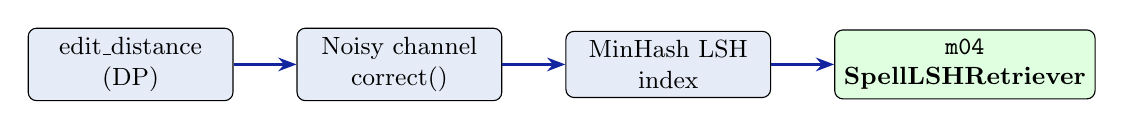
\begin{tikzpicture}[
      mod/.style={draw, fill=cnubluebg, rounded corners=3pt,
                  minimum width=2.6cm, minimum height=0.75cm,
                  font=\small, align=center},
      fin/.style={draw, fill=green!12, rounded corners=3pt,
                  minimum width=2.6cm, minimum height=0.75cm,
                  font=\small\bfseries, align=center},
      arr/.style={-{Stealth}, thick, color=cnublue}
  ]
    \node[mod] (ed)  {edit\_distance\\ (DP)};
    \node[mod, right=0.8cm of ed]  (nc) {Noisy channel\\ correct()};
    \node[mod, right=0.8cm of nc]  (ls) {MinHash LSH\\ index};
    \node[fin, right=0.8cm of ls]  (cap) {\texttt{m04}\\ SpellLSHRetriever};
    \draw[arr] (ed)--(nc);
    \draw[arr] (nc)--(ls);
    \draw[arr] (ls)--(cap);
  \end{tikzpicture}
  \end{center}
  \vspace{5pt}
  \begin{columns}[T]
    \begin{column}{0.50\textwidth}
      \textbf{P4 da qurasiz:}\\[3pt]
      \small
      \begin{itemize}\setlength\itemsep{2pt}
        \item \texttt{edit\_distance(s1, s2)} --- DP jadval
        \item \texttt{correct(word)} --- noisy channel top-nomzod
        \item \texttt{index\_docs} / \texttt{retrieve\_lsh} --- \texttt{datasketch}
        \item k-NN va LSH qidiruv tezligini taqqoslash
      \end{itemize}
    \end{column}
    \begin{column}{0.46\textwidth}
      \textbf{Birinchi assert (bu slayd [I3]):}\\[4pt]
      \small\ttfamily
      assert edit\_distance("qo'l","ko'l")==1\\[4pt]
      \normalfont\footnotesize\color{halfgray}
      \textit{\# Ma'ruza L4 [I3]-slayd bilan}\\
      \textit{\# solishtiring}\\[5pt]
      \normalfont\footnotesize Tayyorlab keling: P3 notebook'ingiz ochiq
      bo'lsin; muhokama savoliga [O] javob.
    \end{column}
  \end{columns}
\end{frame}

% ----------------------------------------------------------------
% [R] ADABIYOTLAR
% ----------------------------------------------------------------
\begin{frame}{Adabiyotlar}
  \begin{enumerate}\small\setlength\itemsep{5pt}
    \item Norvig, P.\ (2009). \textit{How to Write a Spelling Corrector.}
          norvig.com/spell-correct.html
    \item Jurafsky, D., Martin, J.H.\ (2023). \textit{Speech and Language
          Processing}, 3-nashr. 2-bob: Minimum Edit Distance; B-ilova: Spelling.
    \item Levenshtein, V.I.\ (1966). \textit{Binary codes capable of
          correcting deletions, insertions, and reversals.} Soviet Physics Doklady.
    \item Broder, A.\ (1997). \textit{On the resemblance and containment of
          documents.} (MinHash) --- va Indyk \& Motwani (1998), LSH.
    \item \texttt{datasketch} hujjatlari: \texttt{MinHash}, \texttt{MinHashLSH}.
  \end{enumerate}
\end{frame}

% ================================================================
% [S] ILOVALAR (appendix --- slayd soniga kirmaydi)
% ================================================================
\appendix

\begin{frame}{Ilova S1: ``dastur'' va ``dastir'' to'liq DP jadvali}
  \small DP jadval ($s_1=$\texttt{dastur}, $s_2=$\texttt{dastir}):
  \begin{center}\footnotesize
  \begin{tabular}{c|ccccccc}
     & \texttt{""} & \texttt{d} & \texttt{a} & \texttt{s} & \texttt{t} & \texttt{i} & \texttt{r} \\
    \hline
    \texttt{""} & 0 & 1 & 2 & 3 & 4 & 5 & 6 \\
    \texttt{d}  & 1 & 0 & 1 & 2 & 3 & 4 & 5 \\
    \texttt{a}  & 2 & 1 & 0 & 1 & 2 & 3 & 4 \\
    \texttt{s}  & 3 & 2 & 1 & 0 & 1 & 2 & 3 \\
    \texttt{t}  & 4 & 3 & 2 & 1 & 0 & 1 & 2 \\
    \texttt{u}  & 5 & 4 & 3 & 2 & 1 & \textbf{1} & 2 \\
    \texttt{r}  & 6 & 5 & 4 & 3 & 2 & 2 & \textbf{1} \\
  \end{tabular}
  \end{center}
  \vspace{3pt}
  \footnotesize $D[6][6]=1$: faqat \texttt{u}$\to$\texttt{i} almashtirish
  (5-belgi). Diagonal bo'ylab nollar --- mos belgilar.
\end{frame}

\begin{frame}{Ilova S2: MinHash va LSH banding matematikasi}
  \small
  $b$ band, har biri $r$ qatordan ($n=b\cdot r$ xesh). Jaccard $s$ bo'lgan
  juftning kamida bitta bandda to'liq mos kelishi (nomzod bo'lishi) ehtimoli:
  $$ P_{\text{nomzod}}(s) = 1 - (1 - s^{r})^{b} $$
  \bunda{$s$ --- haqiqiy Jaccard; $r$ --- band qatorlari; $b$ --- bandlar soni.}
  \vspace{3pt}

  Bu funksiya $s$ ga nisbatan S-shaklli (sigmoid-simon): $b,r$ ni sozlab,
  ``chegara'' o'xshashlikni (masalan $s\approx 0.5$) tanlash mumkin ---
  undan yuqori juftlar deyarli har doim, pastlari deyarli hech qachon
  nomzod bo'lmaydi.
\end{frame}

\end{document}
